\chapter[Introdução]{Introdução}

\section{Contexto}

A tecnologia tem vindo a evoluir rapidamente e, com isto, nota-se o surgimento de
diversos desafios. Um destes desafios é a falta de programadores que possuam competências 
e qualificação necessárias para solucionar os mais diversos problemas presentes nos mais
variados projetos. Este fato está relacionado com a metodologia adotada no ensino de
programação e também com a falta de motivação por parte dos estudantes \cite{7975788}.

\cite{inproceedings} afirma que, uma das razões de os alunos não absorverem eficientemente
os conceitos relacionados à programação se dá pela falta de concentração e motivação dos mesmos frente
a exposição destes conteúdos na forma tradicional.

\cite{funcional} destaca que a aprendizagem dos conceitos e mecanismos envolvidos na construção de programas não é
trivial, uma vez que requer a utilização de raciocínio na sua forma mais abstrata. Um dos problemas mais comuns segundo os autores
são: dificuldades no entendimento de comandos, sintaxe dos comandos, dificuldades em entender os resultados da execução de um determinado 
comando pela máquina, dificuldades em dar os primeiros passos relativos ao estudo de programação entre outros.

\cite{ambap} diz que, em geral, os alunos têm grandes dificuldades em compreender e aplicar os conceitos relativos à programação . Uma das grandes 
dificuldades está relacionada a problemas de compreensão e aplicação de noções básicas, como por exemplo o uso de estruturas de controle e estruturas
condicionais.

Dificuldades como estas apresentadas, encorajam o desenvolvimento de soluções que auxiliem no ensino e aprendizagem de programação de forma diferente ao
atual modelo de ensino. Diversas abordagens de ensino são estudadas para facilitar o aprendizado dos alunos, algumas delas são:
gamificação, programação imperativa, programação funcional e etc. Neste trabalho, será abordado o uso da gamificação em uma ferramenta
de apoio ao ensino e aprendizagem de programação a ser desenvolvida com base na identificação de requisitos a partir da interação com ex alunos
 e alunos atuais da disciplina de Algoritmos de Programação de Computadores, ofertada pela Universidade de Brasília, campus Gama.

Segundo \cite{6624228}, jogos bem projetados representam bons motivadores, uma vez que passa a sensação de satisfação
e recompensa fazendo com que os jogadores persistam e fiquem engajados em realizar sua missões. Neste contexto, este poder
motivacional dos jogos, passou a ser utilizado em outros contextos que não estão relacionados diretamente aos jogos, uma prática 
conhecida atualmente como Gamificação do inglês \textit{gamification} {\itshape}.

Para \cite{Deterding:2011:GDE:2181037.2181040}, o termo gamificação pode ser definido como a utilização de elementos e mecânica de 
jogos em contextos não relacionados a jogos. De acordo com \cite{Brazil} a utilização destes elementos tornam tarefas reais em atividades
mais atrativas e lúdicas e, consequentemente, aumentam a motivação e engajamento. Há uma grande variedade de ambientes que possuem 
elementos semelhantes a características de jogos, muitos deles contendo: sistema de pontuação, feedbacks constantes e 
etc \cite{6624228}. São exemplos de ambientes com características semelhantes a de jogos: Uri, Datacamp, Edx entre outras.

A aprendizagem baseada na gamificação, preocupa-se em utilizar de mecanismos de jogos não para o entretenimento,
mas para o ensino. Os interessados no campo da gamificação trabalham para identificar o cenário e as condições 
que possam apoiar a integração de jogos aos ambientes de aprendizado. Vários cientistas e estudiosos no campo
da gamificação apontaram uma diversidade de elementos de jogos que permitem que eles sejam utilizados como
ferramentas de apoio ao aprendizado. Por exemplo: os jogos são bastante envolventes \cite{Dickey2005} e motivadores \cite{Prensky:2003:DGL:950566.950596}. Além destas características,
jogos são excelentes fontes para se adquirir experiência que são dificeis de serem fornecidas por meio de instruções tradicionais \cite{Arena2014}.

Os ambientes online gamificados de apoio ao ensino podem fornecer diversas ferramentas, entre elas: classificações, batalhas, fórums de discussões e etc.
De forma a incentivar os usuários a participarem das atividades propostas. 
Durante as competições e batalhas, os estudantes têm a possibilidade de aprender com outros jogadores e comparar suas habilidades, tornando o aprendizado mais
prazeroso \cite{LearningProgramming}. 

\section{Justificativa}

De acordo com \cite{de2009visualg}, a abordagem de ensino tradicional de programação, que é aquela onde o professor apresenta
uma série de conceitos aos alunos e os mesmos têm a tarefa de entender como se aplicam na resolução de problemas,
para a maioria dos estudantes, se revelam muito abstratas.

Um estudo realizado pela Universidade Federal da Paraíba (UFPB) que analisou por seis períodos 
acadêmicos os índices de reprovação na disciplina de Introdução à programação, apontou que 
em nenhum dos seis períodos analisados houvera um índice de aprovação superior a 34\%. Além disso,
os índices de reprovação e trancamento da disciplina giraram em torno dos 64\% e 6\% respectivamente \cite{SBIE6739}.

Um outro estudo, realizado na Faculdade de Educação Tecnológica do Estado do Rio de Janeiro (FAETERJ-Paracambi) por \cite{vieira2015dificuldades}, 
envolvendo 663 alunos da disciplina de Algoritmos 1 mostrou que, destes alunos, apenas 511 cursaram a disciplina 
até o final, ou seja, cerca de 152 alunos desistiram da disciplina. Do total restante (511), apenas 30\% foram
diretamente aprovados (cerca de 153 alunos), 40\% foram reprovados diretamente (204 alunos) e 30\% foram para o exame final (recuperação, 153).
Dos 153 alunos que foram para a recuperação, apenas 55\% foram aprovados (84 alunos), nota-se então que, dos 663 alunos que
foram matriculados na disciplina, apenas  288 alunos foram aprovados ao seu término, cerca de 43\%.

\section{Problema}
Nas seções anteriores, apresentou-se alguns estudos realizados a respeito da situação atual do ensino e aprendizagem
de programação em matérias introdutórias, a partir destes panoramas, o presente trabalho visa responder a seguinte temática
de pesquisa:
Como desenvolver uma ferramenta gamificada para auxiliar o ensino e aprendizagem de programação?
 
\section{Objetivos}
Tendo sido apresentado o contexto e problema que este trabalho visa abranger, objetiva-se
desenvolver uma ferramenta que auxilie professores e estudantes no processo de ensino e aprendizagem
de linguagens de programação em cursos de engenharias.

\chapter{Referencial Teórico}
\section{Gamificação}
Jogos são uma construção humana que envolvem em seu contexto fatores sociais, culturais e econômicos \cite{EaDF440}.

O termo gamificação, segundo \cite{da2014gamificaccao}, consiste na utilização de elementos de jogos em 
atividades que por natureza de sua criação não são jogos. \cite{raposo2016desafio} diz que o objetivo da gamificação, consiste em resolver
problemas práticos ou despertar interesse e engajar um público específico para a realização de uma determinada
atividade. 

\subsection{Gamificação na Educação}
Embora o termo gamificação tenha sido apresentado pela primeira vez em 2010, a idéia de se utilizar
elementos de jogos em atividades que não são jogos, tem sido utilizado há muito tempo. Na educação
 de crianças, por exemplo, as mesmas podiam ter seus esforços e trabalhos reconhecidos por meio
 de estrelinhas ou outros tipos de recompensas dadas por seus educadores, como explica \cite{da2014gamificaccao}.

\subsection{Modelos de Gamificação}
 
\section{Estudos Semelhantes}
Com o objetivo de apoiar o ensino e aprendizado de programação, alguns autores investem no estudo e desenvolvimento
de ferramentas que possam aumentar o interesse e engajamento de alunos. 

\subsection{O Desafio da Serpente}
Tendo em vista os problemas motivacionais e dificuldades enfrentadas por alunos de graduação no que se refere ao
aprendizado de programação do curso de computação da Universidade Federal
da Paraíba, \cite{raposo2016desafio} desenvolveram um jogo que foi disponibilizado na \textit{web} {\itshape} e apelidado
de "O Desafio da Serpente". O propósito da criação do jogo é estimular os alunos a praticarem diariamente seus conhecimentos
por meio de uma série de questões selecionadas e disponibilizadas pelo professor da disciplina.

O jogo envolve os alunos em uma batalha contra uma serpente que faz referência à linguagem de programação utilizada na
disciplina (\textit{python}{\itshape}). Para enfrentar e derrotar a serpente, os jogadores devem conquistar armas mediante o acúmulo
de pontos e resolução dos desafios propostos. 

Em seguida é apresentado um tabuleiro conceitual do jogo. No tabuleiro é possível
identificar por meio das diferentes cores as cinco fases propostas e as armas que podem ser conquistasdas mediante a
resolução dos desafios. O uso do corpo da serpente como tabuleiro tem como objetivo apresentar o caminho sequencial que deve
ser seguido pelos jogadores em busca da vitória. Cada fase, representadas pelas cores na figura \ref{figura1}, correspondem a um conteúdo
que deve ser estudado pelos jogadores.

\begin{figure}[h]
	\centering
	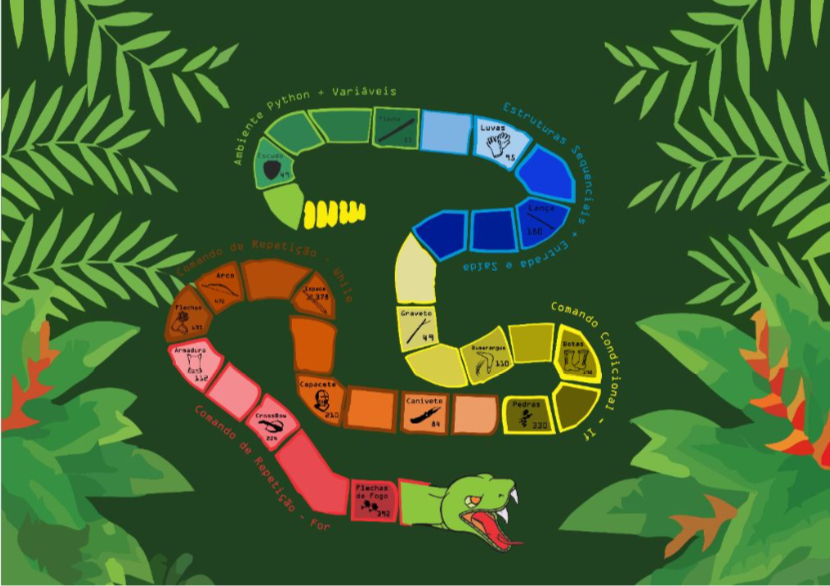
\includegraphics[keepaspectratio=true,scale=0.4]{figuras/desafioSerpente.png}
	\caption{Representação conceitual do jogo}
	\label{figura1}
\end{figure}

Todos os dias da semana, de segunda a sexta feira, eram disponibilizados desafios que continham de duas a seis
questões dos mais variados níveis de complexidade, permitindo que os jogadores, ao concluírem os desafios propostos, 
conquistassem pontos e adquirissem armas, o objetivo era estimular os jogadores a estabelecerem uma rotina de estudos,
dedicando diariamente algum tempo para a resolução de exercícios voltados para a programação.

As questões foram classificadas em três níveis de complexidade (fácil, médio e difícil), no quadro a seguir, apresenta-se
as características de cada um destes níveis.

\begin{table}[h]
	\centering
	\resizebox{\textwidth}{!}{%
	\begin{tabular}{|l|l|l|l|}
	\hline
	\textbf{Complexidade} & \textbf{Tipo de Questão} & \textbf{Tempos estimado para resposta} & \textbf{Quantidade máxima de questões por dia} \\ \hline
	Fácil & \begin{tabular}[c]{@{}l@{}}V ou F\\ Teórica Objetiva\end{tabular} & 5 minutos & 8 \\ \hline
	Médio & \begin{tabular}[c]{@{}l@{}}Acompanhamento\\  (Teste de Mesa)\end{tabular} & 10 minutos & 4 \\ \hline
	Difícil & \begin{tabular}[c]{@{}l@{}}Elaboração de\\ Programas\end{tabular} & 20 minutos & 2 \\ \hline
	\end{tabular}%
	}
	\small{Quadro 1 - Classificação das questões, \cite{raposo2016desafio}} 
\end{table}

Objetivando manter os jogadores motivados, cada fase possuia um sistema de (\textit{ranking}{\itshape}) independente
das fases anteriores, desta forma, mesmo que um jogador não tenha obtido uma boa pontuação nas fases anteriores, ele
começaria a fase seguinte sem desvantagem em relação aos demais jogadores. 

A medida que os jogadores acumulavam pontos, os mesmos conquistavam novas armas para combater a serpente. Estas armas podiam
ser de defesa(escudos,armaduras e etc) ou de ataque(espada, lança e etc). O objetivo era que os jogadores conseguissem conquistar
o maior número possível de armas em cada fase. Cada armamento possuia uma quantidade mínima de pontos necessários para sua
aquisição e possuiam apenas características simbólicas.

\begin{figure}[h]
	\centering
	
\includegraphics[keepaspectratio=true,scale=0.4]{figuras/armas.png}
	\caption{Exemplos de armas e pontuações, \cite{raposo2016desafio}}
	\label{figura1}
\end{figure}

Além de permitir os jogadores colecionarem pontos e armas, os primeiros jogadores tinham sua fotos expostas no
site do jogo, exaltando suas conquistas.

Para motivar os alunos a utilizarem a ferramenta e possibilitar a coleta de dados que
permitissem analisar o impacto do uso da tecnologia gamificada no ensino de programação, foi 
acordado que, os alunos que obtivessem um aproveitamento de no mínimo 70\% em todas as fases do jogo,
receberiam um ponto extra na primeira unidade da disciplina. Os alunos que obtivessem nota superior ou igual 
a 50\% em todas as fases do jogo, receberiam meio ponto extra na nota da primeira unidade da disciplina.
Desta forma, a participação no jogo teria caráter voluntário, e não estaria diretamente ligada às avaliações da 
disciplina. Recompensar os alunos com pontos extras tinha como objetivo  
identificar até que ponto a motivação dos jogadores em resolver os desafios era ocasionado pelo próprio jogo e não 
pelos pontos.

Considerando as quatro primeiras semanas de aula utilizando a ferramenta, os resultados foram bastante animadores.
Dos total 106 alunos que realmente frequentaram as aulas, apenas quatro não participaram de nenhum 
dos desafios propostos, o que indica que a aceitação da ferramenta pelos alunos foi de mais de 96\%. Além destes indicadores
quantitativos, \cite{raposo2016desafio} relatou em sua pesquisa que a empolgação dos alunos na utilização da ferramenta
era bastante perceptível. Muitos alunos se diziam bastante ansiosos para o desafio do dia e notou-se um grande aumento 
no número de discussões a respeito das questões durante as aulas.

\chapter{Metodologia}

\begin{itemize}
	\item Levantamento de requisitos (questionários, literatura, ferramentas semelhantes, plano de ensino, currículo pedagógico e etc) -> tabelar
	\item Priorização de requisitos (usar o moscow?)
	\item Entrevistas (entrevistar colegas que já fizeram e estão fazendo)
	\item Conversas com professores
\end{itemize}

\section{Desenvolvimento}

\subsection{Arquitetura}


\subsection{Ferramentas}

Para o desenvolvimento de uma solucão de software, deve-se considerar diversos
fatores, como: afinidade com as tecnologias de auxílio ao desenvolvimento, recursos disponibilizados pela tecnologia 
(frameworks, bibliotecas e etc), documentação da tecnologia entre outros fatores que podem influenciar diretamente
na construção do sistema.

No desenvolvimento desta ferramenta, a mesma foi dividida em duas áreas principais: backend e frontend. Para cada uma destas
áreas, apresentamos a seguir as ferramentas utilizadas.

